\chapter{Model}

\section{Cahn Hilliard Model}
Cahn–Hilliard Model for a compositionally inhomogeneous alloy is used. It is developed using the composition field \textbf{c(r)} in an alloy. The local composition \textbf{c} used in this model is defined as follows: 

\begin{equation}
\mathbold{
\frac{c^{'}-c^{'}_{\alpha}}{c^{'}_{\beta}-c^{'}_{\alpha}}
}
\end{equation}

where, $\mathbold{c^{'}}$ is the local composition,\\
$\mathbold{c^{'}_{\alpha}}$ is the equilibrium composition of the A rich $\mathbold{\alpha}$ phase,\\
$\mathbold{c^{'}_{\beta}}$ is the equilibrium composition of the B rich $\mathbold{\beta}$ phase,\\
all the above values are expressed in mole fraction of species B. Thus, for $\mathbold{\alpha}$ phase $\mathbold{c = 0}$ and for $\mathbold{\beta}$ phase $\mathbold{c = 1}$


\section{Cahn Allen Model}
Cahn–Allen theory for non-conserved variables (the model of Fan and Chen (1997) belongs to this category) is used. It is developed using a set of \textbf{n} 'orientational' (and non-conserved) order parameter fields $\mathbold{\eta_{i}(r) (i =1,2,...,n) }$to represent \textbf{n} different grain orientations in the microstructure; $\mathbold{\eta_{i}}$ are continuum analogues of Potts variables in the \textbf{n}-state Potts model

Each $\mathbold{\eta_{i}}$ is taken to be 1 within the $i^{th}$ grain and drops
to 0 outside it, through a GB region where it varies smoothly.

\begin{figure}[H]
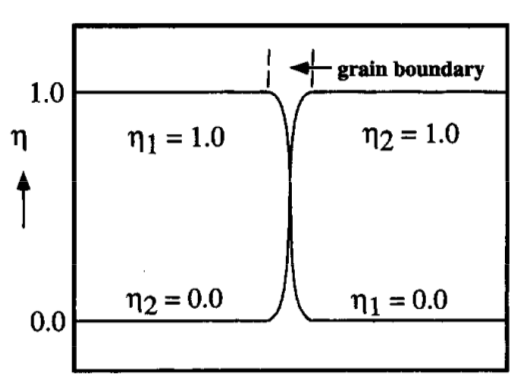
\includegraphics[scale=0.7]{gbProfile}
\caption{The schematic profiles of two orientation variables across a flat grain boundary}
\end{figure}

\section{Conclusion}
An instantaneous configuration in our model is described in terms of the \textbf{n+1} position-dependent field variables $\mathbold{(c;\eta_1, \eta_2, …….., \eta_n)}$.

